\section{Discussion}\label{sec:discussion}
\subsection{Traveling standing waves at normal incidence}

Change the absorbing boundary in the second medium to a perfect electric boundary.

\paragraph{Task 2a} \textit{Identify the standing and traveling wave in the structure.}
\begin{figure}[tbph]
	\centering
	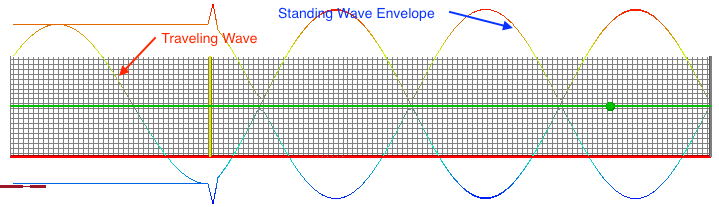
\includegraphics[width=0.95\linewidth]{graphics/Task2-2a-Standing-better-envelope}
	\caption{Standing wave pattern for waveguide with electric boundary at right end}
	\label{fig:Task2-2a-Standing-better-envelope}
\end{figure}

\pagebreak
\paragraph{Task 2b} \textit{What is the amplitude of the wave at the probe? Is it \SI{2}{\volt\per\meter}? Why?}
\begin{figure}[tbph]
	\centering
	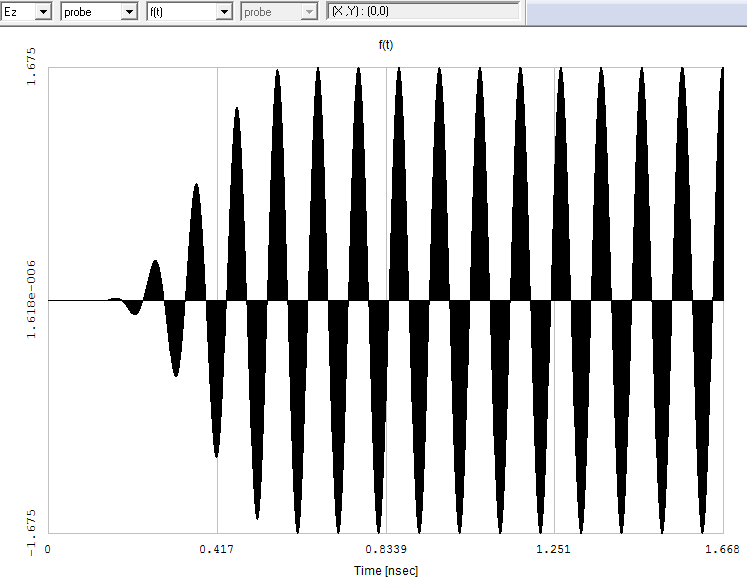
\includegraphics[width=0.6\linewidth]{graphics/Task2-2b-Amplitude}
\end{figure}

The amplitude of the standing wave is \SI{1.675}{\volt\per\meter} because the probe is not located at a standing wave antinode: odd integer multiples of $l_{max}$.

\paragraph{Task 2c} \textit{What is the amplitude of the wave to the left of the source region? Is it \SI{2}{\volt\per\meter}? Why?}

Fig.~\ref{fig:Task2-2a-Standing-better-envelope} shows that the wave has an amplitude of \SI{2}{\volt\per\meter}.
This is because the reflected wave is in phase with the source wave at the wave origin and constructive interference occurs.

\paragraph{Task 2d} \textit{What are: $E_{max}, E_{min}, l_{max}, l_{min}, \left|\Gamma\right|, \phi_\Gamma$? What are possible sources of error between the simulation and expected values?}
\begin{table}[htpb]
	\centering
	\begin{tabular}{@{}ccc@{}}
		\toprule
		Parameter             & Expected                & Actual \\ 
		\midrule
		$E_{max}$             & \SI{2}{\volt\per\meter} & \SI{1.969}{\volt\per\meter} \\
		$E_{min}$             & \SI{0}{\volt\per\meter} & \SI{0.3478}{\volt\per\meter} \\
		$l_{max}$             & \SI{62.5}{\milli\meter} & $<62.5$\si{\milli\meter} \\
		$l_{min}$             & \SI{55}{\milli\meter}   & $<55$\si{\milli\meter} \\
		$\left|\Gamma\right|$ & \sfrac{1}{3}            & \sfrac{1}{3} \\
		$\phi_\Gamma$         & $-\pi$~\si{\radian}     & $-\pi$~\si{\radian} \\ 
		\bottomrule
	\end{tabular}
\end{table}

The values of $E$ differ from the expected values because the probes for those measurements were placed at the positions of $l_{max}$ and $l_{min}$ as determined by calculating the wavelength for $c_0 = \SI{3.0E8}{\meter\per\second}$.

\pagebreak
\paragraph{Task 5a} \textit{Set $\epsilon_{r2} = 4$, $\sigma_2 = \SI{1}{\siemens\per\meter}$ and repeat Task 2 with an absorbing right boundary.}
\begin{figure}[tbph]
	\centering
	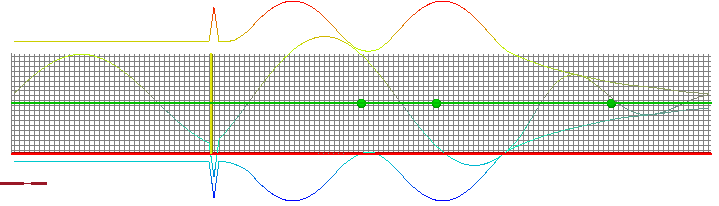
\includegraphics[width=0.95\linewidth]{graphics/Task2-5a-Standing}
	\caption{$\epsilon_{r2} = 4$, $\sigma_2 = \SI{1}{\siemens\per\meter}$, absorbing right boundary}
	\label{fig:Task2-5a-Standing}
\end{figure}

A standing wave envelope is produced between the source and dielectric boundary.
As the wave enters the second medium it is attenuated.

\paragraph{Task 5b} \textit{What is the amplitude of the wave at the probe? Is it \SI{2}{\volt\per\meter}? Why?}
\begin{figure}[tbph]
	\centering
	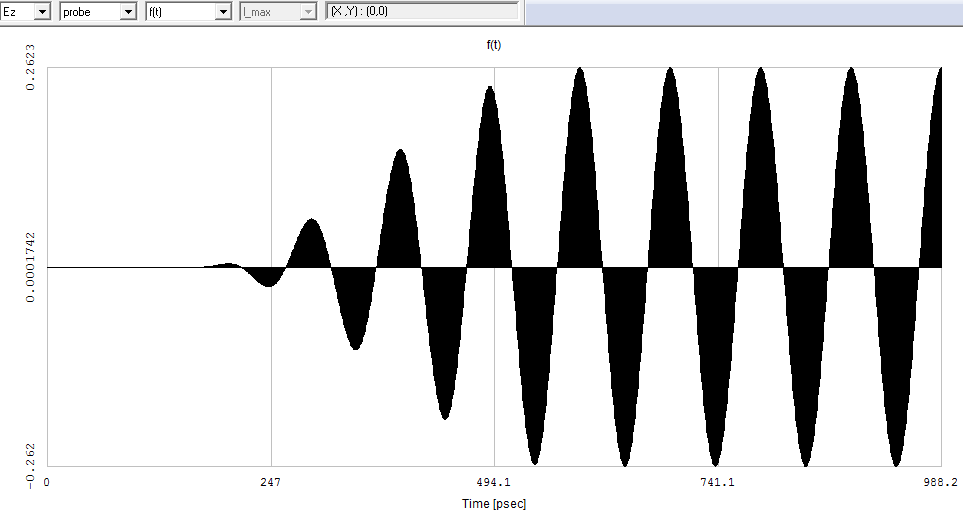
\includegraphics[width=0.6\linewidth]{graphics/Task2-5b-Amplitude}
\end{figure}

The amplitude is \SI{0.263}{\volt\per\meter}.
As noted in 2b, the source is not placed at an antinode.
Also, the wave attenuates as it enters the second medium because $\sigma_2 \ne 0$.

\pagebreak
\paragraph{Task 5c} \textit{What is the amplitude of the wave to the left of the source region? Is it \SI{2}{\volt\per\meter}? Why?}

\begin{figure}[tbph]
	\centering
	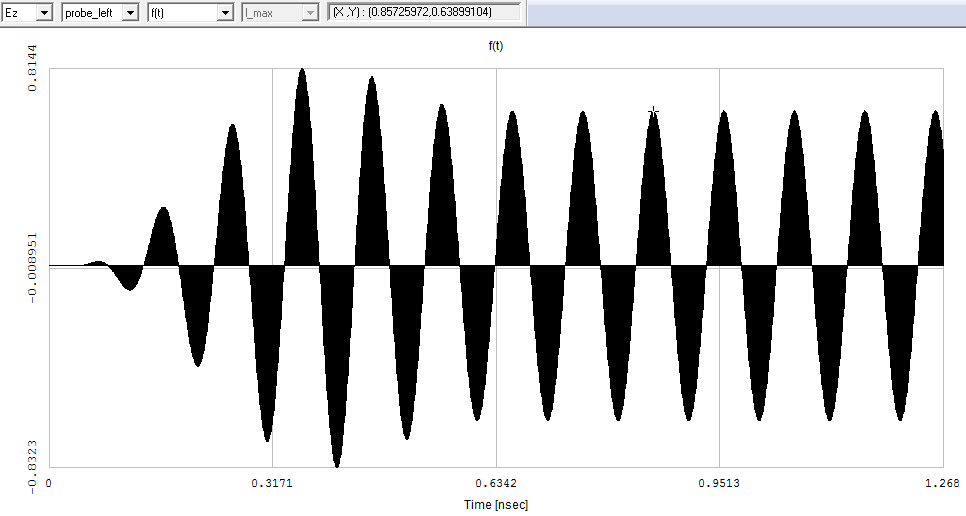
\includegraphics[width=0.6\linewidth]{graphics/Task2-5c-Amplitude_left}
\end{figure}
The amplitude is \SI{0.639}{\volt\per\meter}, which is close to the value of $E_{min}$. This is because destructive interference occurs when the wave reaches the source origin.

\paragraph{Task 5d} \textit{What are: $E_{max}, E_{min}, l_{max}, l_{min}, \left|\Gamma\right|, \phi_\Gamma$? What are possible sources of error between the simulation and expected values?}
\begin{table}[htpb]
	\centering
	\begin{tabular}{@{}ccc@{}}
		\toprule
		Parameter             & Expected                   & Actual \\ 
		\midrule
		$E_{max}$             & \SI{1.33}{\volt\per\meter} & \SI{1.365}{\volt\per\meter} \\
		$E_{min}$             & \SI{0.67}{\volt\per\meter} & \SI{0.6414}{\volt\per\meter} \\
		$l_{max}$             & \SI{42.5}{\milli\meter}    & $>42.5$\si{\milli\meter} \\
		$l_{min}$             & \SI{50}{\milli\meter}      & $>50$\si{\milli\meter} \\
		$\left|\Gamma\right|$ & \sfrac{1}{3}               & 0.36 \\
		$\phi_\Gamma$         & $-\pi$~\si{\radian}        & $-\pi$~\si{\radian} \\ 
		\bottomrule
	\end{tabular}
\end{table}

Again, error comes from approximating $c_0$.

\pagebreak
\paragraph{Task 6a} \textit{Set $\epsilon_{r1} = 9$, $\sigma_1 = \SI{0.5}{\siemens\per\meter}$ and repeat Task 5.}
\begin{figure}[tbph]
	\centering
	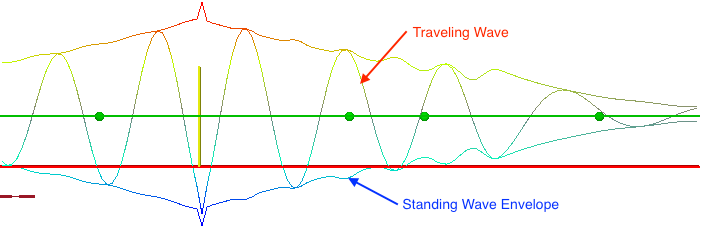
\includegraphics[width=0.96\linewidth]{graphics/Task2-6a-Standing}
	\caption{$\epsilon_{r1} = 9$, $\sigma_1 = \SI{0.5}{\siemens\per\meter}$, $\epsilon_{r2} = 4$, $\sigma_2 = \SI{1}{\siemens\per\meter}$}
	\label{fig:Task2-6a-Standing}
\end{figure}

The wave attenuates in the first dielectric because $\sigma_1 \ne 0$.

\paragraph{Task 6b} \textit{What is the amplitude of the wave at the probe? Is it \SI{2}{\volt\per\meter}? Why?}
\begin{figure}[tbph]
	\centering
	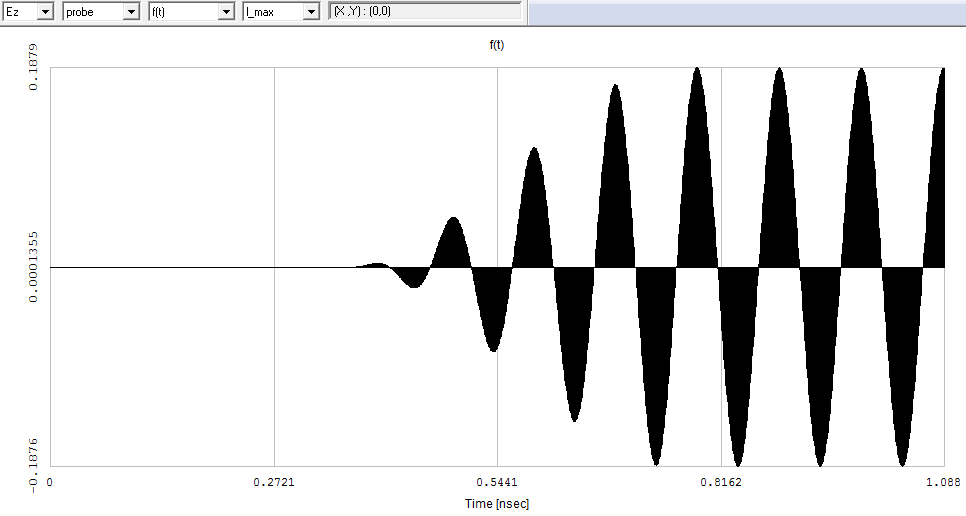
\includegraphics[width=0.6\linewidth]{graphics/Task2-6b-Amplitude}
\end{figure}

The amplitude is \SI{0.1879}{\volt\per\meter}.
It is smaller than in 5b because the wave attenuated in the first medium.

\pagebreak
\paragraph{Task 6c} \textit{What is the amplitude of the wave to the left of the source region? Is it \SI{2}{\volt\per\meter}? Why?}
\begin{figure}[tbph]
	\centering
	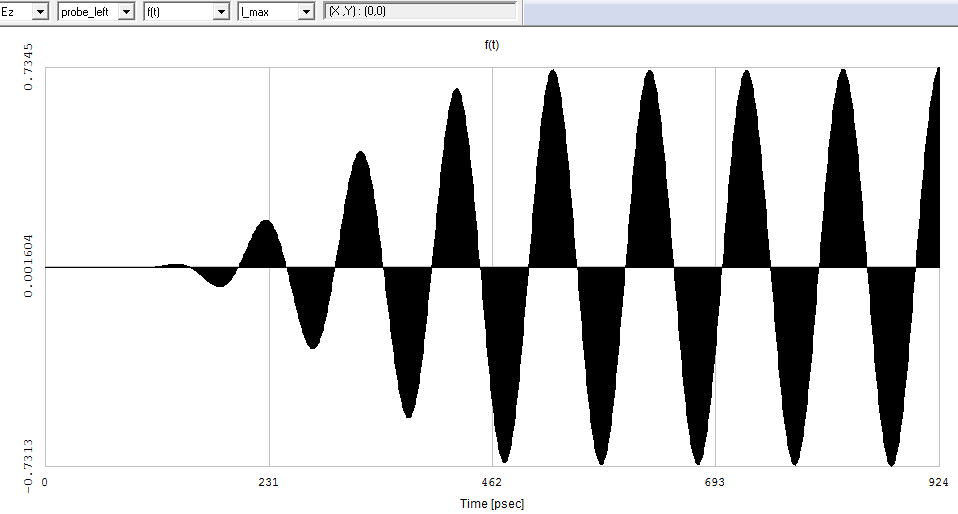
\includegraphics[width=0.6\linewidth]{graphics/Task2-6c-Amplitude_left}
\end{figure}

The amplitude is \SI{0.7345}{\volt\per\meter} at the location of the leftmost probe in Fig.~\ref{fig:Task2-6a-Standing}.
At the location just to the left of the source it has an amplitude of \SI{1}{\volt\per\meter}.
Since the reflected wave is \SI{90}{\degree} out of phase it does not receive constructive or destructive interference.

\paragraph{Task 6d} \textit{What are: $E_{max}, E_{min}, l_{max}, l_{min}, \left|\Gamma\right|, \phi_\Gamma$? What are possible sources of error between the simulation and expected values?}
\begin{table}[htpb]
	\centering
	\begin{tabular}{@{}ccc@{}}
		\toprule
		Parameter             & Expected                   & Actual \\ 
		\midrule
		$E_{max}$             & \SI{0.749}{\volt\per\meter} & \SI{0.6587}{\volt\per\meter} \\
		$E_{min}$             & \SI{0.436}{\volt\per\meter} & \SI{0.4573}{\volt\per\meter} \\
		$l_{max}$             & \SI{42.5}{\milli\meter}    & $>42.5$\si{\milli\meter} \\
		$l_{min}$             & \SI{50}{\milli\meter}      & $>50$\si{\milli\meter} \\
		$\left|\Gamma\right|$ & 0.20 & 0.18 \\
		$\phi_\Gamma$         & 0~\si{\radian} & 0~\si{\radian} \\
		\bottomrule
	\end{tabular}
\end{table}

Error is introduced in the calculation of $\left|\Gamma\right|$ because measurements of successive nodes and antinodes to find the SWR does not account for the effect of attenuation. This causes SWR to be larger than expected, thus $\left|\Gamma\right|$ is smaller than expected.
A similar error is introduced when calculating $E_{max}$ and $E_{min}$.

\pagebreak
\paragraph{Task 8} \textit{Design an impedance transformer with minimum thickness so that a 7.5 GHz wave can pass through without reflection.}

\begin{figure}[tbph]
\centering
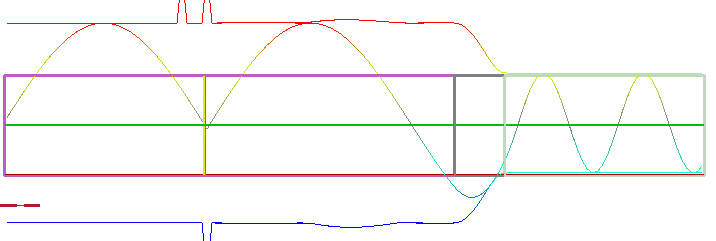
\includegraphics[width=0.95\linewidth]{graphics/Task3-8-Standing_5mm}
\caption{Impedance tranformer with $\epsilon_{r2} = 4$ and $d = \SI{5}{\milli\meter}$}
\label{fig:Task3-8-Standing_5mm}
\end{figure}

For this configuration, $\epsilon_{r1} = 1$ and $\epsilon_{r3} = 16$. Thus
\begin{equation*}
	\epsilon_{r2} = \sqrt{\epsilon_{r1}\epsilon_{r3}} = 4
\end{equation*}
and
\begin{equation*}
	d = {\lambda_2 \over 4} = {c_0 \over 4 \sqrt{\epsilon_{r2}} f} \approx \SI{5}{\milli\meter}.
\end{equation*}

\paragraph{Task 10} \textit{Modify the impedance transformer from Task 8 to the third minimum thickness.}

\begin{figure}[tbph]
	\centering
	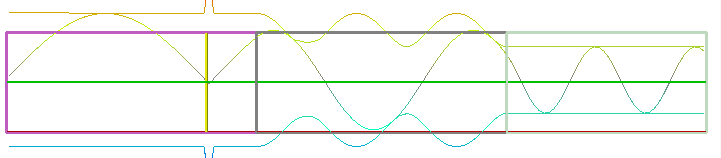
\includegraphics[width=0.95\linewidth]{graphics/Task3-10-Standing_25mm}
	\caption{Impedance tranformer with $\epsilon_{r2} = 4$ and $d = \SI{25}{\milli\meter}$}
	\label{fig:Task3-8-Standing_25mm}
\end{figure}

Successive impedance transformers can be created by adding integer multiples of \sfrac{$\lambda_2$}{2}.

\pagebreak
\paragraph{Task 11 \& 12} \textit{Set $\epsilon_{r1} = 2$ and $\epsilon_{r3} = 8$ and perform simulations for 6.5, 7.5, 8.5 GHz.}

\begin{figure}[htpb]
	\centering
	\subfigure[$f = \SI{6.5}{\giga\hertz}$, $d = \SI{5.8}{\milli\meter}$]
	{
		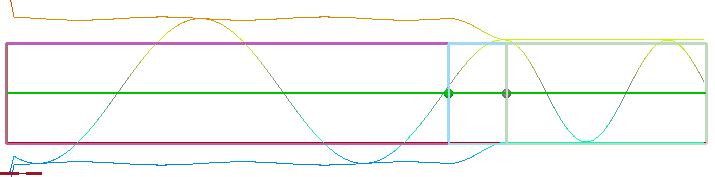
\includegraphics[width=0.95\linewidth]{graphics/Task3-11-6,5GHz_Standing_5,8mm}
		\label{sfig:6.5GHz}
	}
	\subfigure[$f = \SI{7.5}{\giga\hertz}$, $d = \SI{5}{\milli\meter}$]
	{
		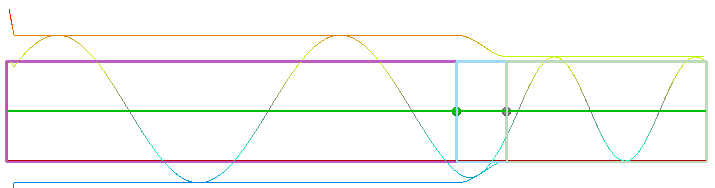
\includegraphics[width=0.95\linewidth]{graphics/Task3-11-7,5GHz_Standing_5mm.png}
		\label{sfig:7.5GHz}
	}
	\subfigure[$f = \SI{8.5}{\giga\hertz}$, $d = \SI{4.41}{\milli\meter}$]
	{
		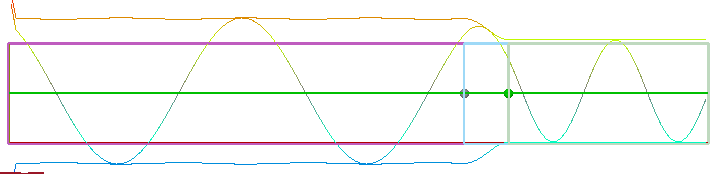
\includegraphics[width=0.95\linewidth]{graphics/Task3-11-8,5GHz_Standing_4,41mm.png}
		\label{sfig:8.5GHz}
	}
	\caption{Impedance transformers for $\epsilon_{r1} = 2$ and $\epsilon_{r3} = 8$}
	\label{fig:Task11}
\end{figure}

As for Task 8, $\epsilon_{r2} = 4$ and $d$ is a quarter wavelength in material 2.

\begin{table}[htpb]
	\centering
%	\caption{My caption}
%	\label{my-label}
	\begin{tabular}{@{}cccc@{}}
		\toprule
		Parameter & 6.5 GHz & 7.5 GHz & 8.5 GHz \\ \midrule
		$E_{max}$ & \SI{1.001}{\volt\per\meter} & \SI{0.9979}{\volt\per\meter} & \SI{0.9988}{\volt\per\meter} \\
		$E_{min}$ & \SI{0.7055}{\volt\per\meter} & \SI{0.7062}{\volt\per\meter} & \SI{0.7061}{\volt\per\meter} \\
		$l_{max}$ & \SI{44.2}{\milli\meter} & \SI{45}{\milli\meter} & \SI{45.59}{\milli\meter} \\
		$l_{min}$ & \SI{50}{\milli\meter} & \SI{50}{\milli\meter} & \SI{50}{\milli\meter} \\
		$\left|\Gamma\right|$ & 0.176 & 0.176 & 0.176 \\
		$\phi_\Gamma$ &  $-\pi$~\si{\radian} & $-\pi$~\si{\radian} & $-\pi$~\si{\radian} \\ \bottomrule
	\end{tabular}
\end{table}

\subsection*{Sample calculations}
\begin{align*}
	\left|\Gamma\right| = {SWR - 1 \over SWR + 1} = {\frac{1}{0.7} - 1 \over \frac{1}{0.7} + 1 } = {0.4286 \over 2.4286} = 0.176
\end{align*}
\begin{align*}
	\phi_\Gamma = - \pi - {4 \pi \over \lambda}z_{min} = - \pi - {4 \pi \over \lambda}(0) = -\pi
\end{align*}

This transformation can be shown on a Smith chart:

\begin{figure}[tbph]
\centering
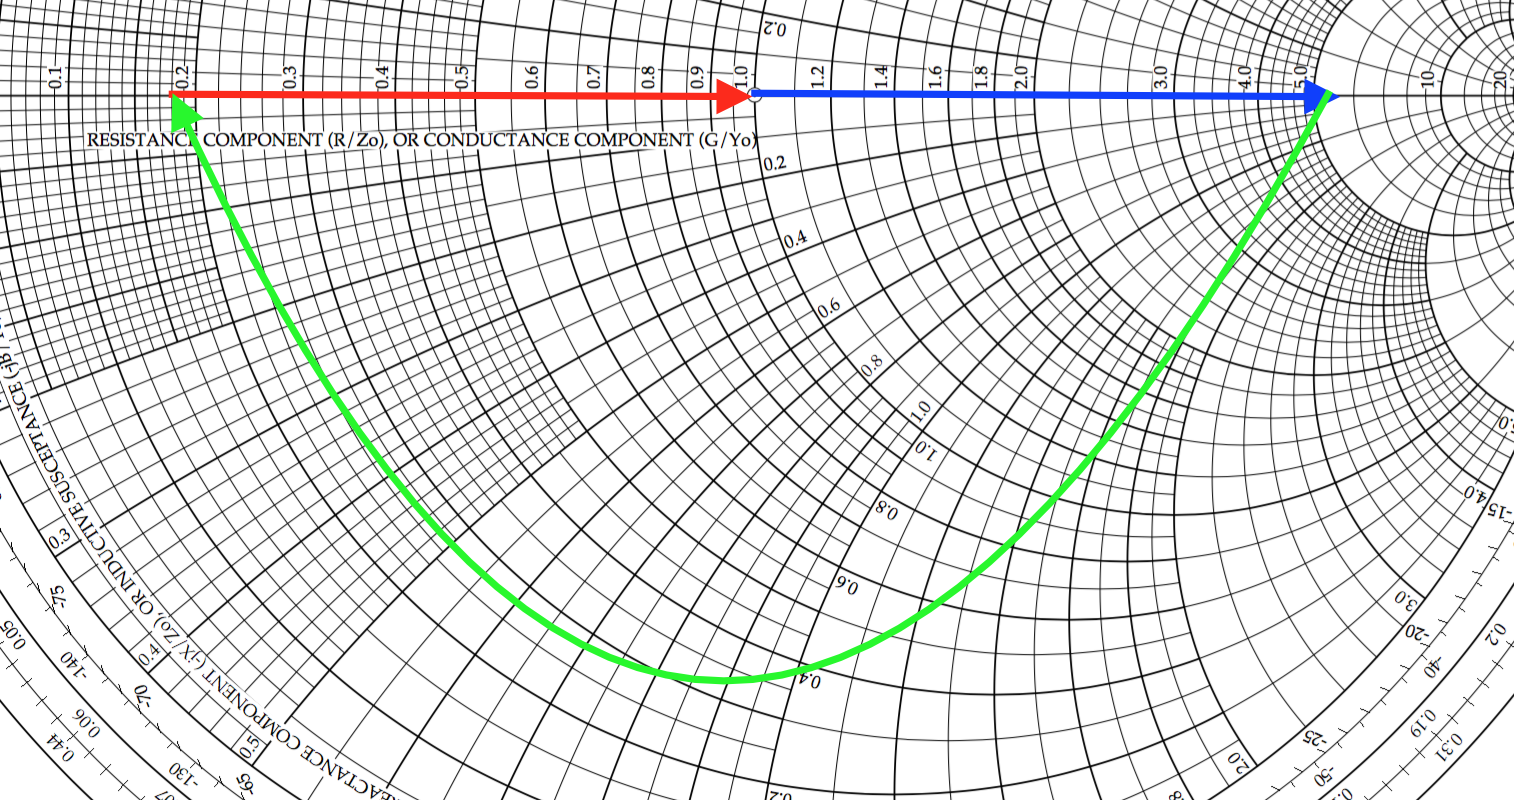
\includegraphics[width=0.7\linewidth]{graphics/Task3-12-Smith}
\label{fig:Smith}
\end{figure}

The blue arrow shows the material 2 to 3 transition; the green arrow shows the wave moving through a quarter wavelength of material 2, and; the red arrow show the material 1 to 2 transition.

Since all three frequencies have the same values for $\left|\Gamma\right|$ and relative permittivities, the Smith charts are identical.
